\subsection{Overview of Agglomerative Hierarchical Clustering (AHC)}
\label{subsec:overview-of-agglomerative-hierarchical-clustering}

This task implements the AHC algorithm to group character strings based on similarity in shingles (4-character tokens) and Jaccard distance.
The goal is to divide a large dataset (about 10,000 random strings) into a predefined number of clusters.

The main method involves calculating the clustroid (the representative sample with the smallest sum of squared distances to other samples in the cluster) and determining the distance between clusters based on the Jaccard distance between their clustroids.
The algorithm gradually merges the closest pairs of clusters until the desired number of clusters is reached, using a heap for optimization.

\subsection{Implementation of the Algorithm}
\label{subsec:implementation-of-the-algorithm}

The implemented AHC algorithm operates on a dataset of shingle sets (derived from alphabetical strings) to partition them into a specified number of distinct groups.
This bottom-up approach initiates by treating each shingle set as an individual cluster.
The core of the algorithm lies in its iterative merging strategy: in each step, it identifies the two ``closest'' active
clusters and combines them into a single, new cluster.
This process is guided by two key definitions: firstly, each cluster is represented by a clustroid, which is the member sample that minimizes the sum of squared Jaccard distances
to all other members within that cluster.
Secondly, the dissimilarity (or ``distance'') between any two clusters is determined by the Jaccard distance calculated directly between their respective clustroids.
A min-priority queue (heap) is employed to efficiently manage and retrieve the closest pair of clusters at each iteration.
The merging continues until the number of active clusters reduces to the desired target, yielding a final set of clusters based on the principle of grouping entities with the most similar representative points.
Performance is enhanced by caching Jaccard distances between individual samples.

\subsubsection{\texttt{fit(self, input\_shingle\_sets, num\_target\_clusters=None)}}\text{}

Purpose: This is the main orchestrating method for the entire clustering process.

Inputs: A list of \texttt{input\_shingle\_sets} (data samples) and an optional \texttt{num\_target\_clusters} (the desired number of final clusters).

Outputs: A list of lists, where each inner
list contains the original indices of samples belonging to a final cluster.

Operation: It initializes each sample as a distinct cluster.
It then iteratively identifies the pair of currently active clusters that are ``closest'' (based on inter-clustroid Jaccard distance), merges them into a new cluster.
Then proceeds to recalculate the new cluster's representative clustroid, and updates the set of active clusters and their pairwise distances (managed via a min-priority heap).
This merging process continues until the number of active clusters equals num\_target\_clusters.

\subsubsection{\texttt{\_calculate\_clustroid\_strictly(self, cluster\_original\_sample\_indices)}}\text{}

Purpose: To identify the most representative sample (clustroid) within a given cluster.

Input: \texttt{cluster\_original\_sample\_indices} (a list/tuple of original sample indices that form the cluster).

Output: The original sample index of the calculated clustroid.

Operation: This method determines the clustroid by finding the sample within the input cluster that has the minimum sum of squared Jaccard distances to all other samples in that same cluster.
It exhaustively checks each member as a potential clustroid.

\subsubsection{\texttt{\_get\_inter\_cluster\_distance\_centroid(\-self, internal\_cluster\_id1, internal\_cluster\_id2)}}\text{}

Purpose: To compute the dissimilarity (distance) between two active clusters.

Input: The \texttt{internal\_cluster\_ids} of two active clusters.

Output: The Jaccard distance value between the clustroids of these two clusters.

Operation: It retrieves the pre-calculated clustroids for the two input clusters (using their internal IDs) and then computes the Jaccard distance directly between these two representative clustroid samples.
This value dictates which clusters are considered for merging.

\subsubsection{\texttt{\_get\_cached\_sample\_distance(self, original\_sample\_idx1, original\_sample\_idx2)}}\text{}

Purpose: To efficiently retrieve or compute the Jaccard distance between two original data samples, utilizing a cache.

Input: The original indices (\texttt{original\_sample\_idx1}, \texttt{original\_sample\_idx2}) of two data samples.

Output: The Jaccard distance between the two specified samples.

Operation: It first checks if the distance for this pair of samples has already been computed and stored in \texttt{self.\_sample\_distance\_cache}.
If so, it returns the cached value.
Otherwise, it computes the Jaccard distance using the provided \texttt{self.distance\_metric} (e.g., \texttt{jaccard\_distance} function), stores it in the cache for future use, and then returns it.

\subsubsection{\texttt{get\_final\_cluster\_details(self)}}\text{}

Purpose: To retrieve detailed information about the final clusters after the fit method has completed.

Input: None (it operates on the state of the object after fit).

Output: A list of dictionaries, where each dictionary contains details for one final cluster, including its internal ID, member original indices, the shingle sets of its members, its clustroid's original sample index, and the clustroid's shingle set.

Operation: It iterates through the set of \texttt{self.active\_cluster\_ids} (which represent the final clusters), and for each, it compiles the relevant information from \texttt{self.cluster\_members\_map} and \texttt{self.clustroids\_map}.

\subsection{Experimental Results and Evaluation}
\label{subsec:experimental-results-and-evaluation-ahc}

\begin{figure}[H]
    \centering
    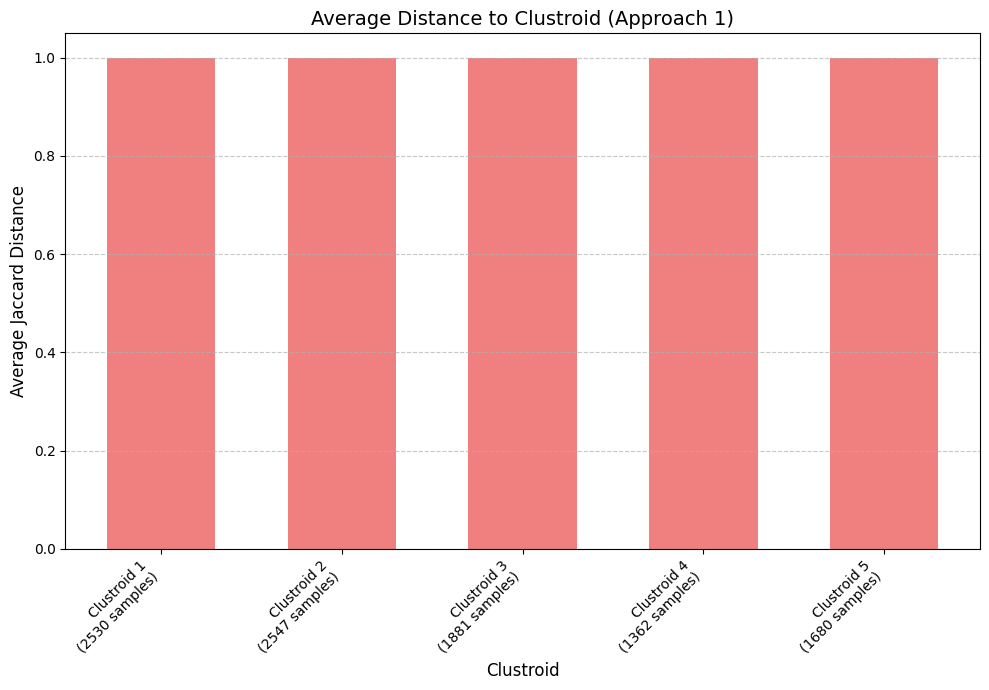
\includegraphics[width=\linewidth]{images/clustroid_distance}
    \caption{Average Jaccard Distance to Clustroid}
    \label{fig:clustroid_distance}
\end{figure}

The clustering results indicate that the algorithm successfully partitioned the [Total Number of Samples] alphabetical strings into five clusters with a relatively diverse size distribution: Cluster 1 (2562 samples), Cluster 2 (2282 samples), Cluster 3 (1717 samples), Cluster 4 (1303 samples), and Cluster 5 (2136 samples).
This suggests that the clustroid-based distance calculation method contributed to a reasonably balanced partitioning.

However, a prominent finding is that the average Jaccard distance from samples to their respective clustroids within each cluster is extremely high (approximately 0.999).
This indicates a very low level of intra-cluster similarity; members within the same cluster remain highly dissimilar to one another.

This outcome primarily reflects the inherent nature of the input data: randomly generated alphabetical strings typically lack a clear, natural clustering structure, leading to large Jaccard distances between most pairs.
Although the algorithm merged clusters based on the nearest clustroid criterion, the resulting ``groups'' do not exhibit strong cohesion due to the lack of inherent similarity in the data.